%\subsubsection{Quark/Gluon jets uncertainty}
\label{subsec:bkg_uncer_qg}

Jet flavor response and composition uncertainties consider the different jet responses to quark- and gluon-initiated jets. 
The response uncertainties are centrally derived from dijet events using alternative MC samples, specifically Pythia 8 and Herwig++. 
For flavor composition, uncertainties are typically assumed based on a 50/50 quark/gluon mix, with a conservative (100\%) uncertainty. 
However, in VBS topologies, which tend to be quark-enriched, such uncertainties can limit measurement sensitivity. 
To mitigate this, we study the gluon fraction within our analysis phase-space. 
This allows us to rederive jet flavor-related uncertainties using custom gluon fractions, thus potentially reducing these uncertainties.

The estimation of the gluon fraction across various analysis regions and samples is performed as a function of the small-\(R\) jet \(\pt\) and \(\eta\). This is achieved by utilizing truth parton label information to discern the quantity of quarks and gluons. For the purpose of quark estimation, all jets are considered in the denominator, with the exception of those initiated by b-quarks.

The gluon fraction for each analysis region and across various samples is calculated based on the small-$R$ jet $\pt$ and $\eta$. 
This estimation utilizes truth parton label information to determine the number of quarks and gluons. 
For the purpose of quark estimation, all jets except those initiated by $b$-quarks are considered in the denominator.

Two-dimensional histograms, representing the gluon fraction as a function of jet $\pt$ and $\eta$, serve as inputs for recalculating jet flavor and composition uncertainties. Each MC sample is associated with a single input file. 
The gluon fraction for a specific ($\pt$, $\eta$) bin is determined by aggregating data across all regions, according to the nominal approach.

To account for the uncertainty in the gluon fraction, additional inputs are utilized. The uncertainty for a particular ($\pt$, $\eta$) bin, $\sigma_{gfrac}$, is calculated as follows:
\[
\sigma_{gfrac} = \sqrt{\sigma_{region}^{2} + \sigma_{gen}^{2}}
\]
Here, \(\sigma_{region}\) represents the maximal deviation in gluon fraction between the nominal and any analysis region. Meanwhile, \(\sigma_{gen}\) denotes the generator uncertainty, obtained from comparing alternative Pythia 8 and Herwig++ MC samples.


The inputs for the gluon fraction and their corresponding uncertainties in the \olep channel are illustrated in Figures \ref{fig:QGFracInputs2D1Lep} and \ref{fig:QGFracErrorInputs2D1Lep}, respectively. 
Comparison between old flavor uncertainties and newly derived flavor uncertainties is shown is Figure \ref{fig:1LepFlavorVarOldNew}. It is evident from this comparison that flavor composition uncertainties, in general, are reduced.


%%%%%%%%
%%%The jet flavor response and composition uncertainties account for the different jet responses to quark- and gluon-initiated jets. The flavor response uncertainties are derived centrally from dijet events using alternative (Pythia 8 and Herwig++) Monte Carlo. Flavor composition uncertainties are usually derived assuming a 50/50 quark/gluon composition with a very conservative (100\%) uncertainty. In VBS topologies where quark enriched regions are expected such uncertainties can limit the sensitivity of the measurement. In order to reduce such uncertainties, the gluon fraction in our analysis phase-space is studied and jet flavor related uncertainties are rederived using custom gluon fractions. %anastasia; Maybe add formulas for jet flavour composition and jet flavour response from dimitris lectures
%%%
%%%The gluon fraction in each of the analysis regions and for the different analysis samples is estimated as a function of the small-$R$ jet $\pt$ and $\eta$. Truth parton label information is used in order to estimate the number of quarks and gluons.  All jets except b-quark-initiated jets are included in the denominator for the quark estimation. 
%%%
%%%In Figures \ref{fig:2lep_gfrac_pt} and  \ref{fig:2lep_gfrac_eta} a comparison of the gluon fraction between the different analysis regions for the 2-lepton channel main MC samples is plotted as a function of $\pt$ and $\eta$ respectively. A clear $\pt$ and $\eta$ dependence of the gluon fraction is noticed.
%%%
%%%2D histograms of the gluon fraction as a function of  $\pt$ and $\eta$ are used as inputs to recalculate the jet flavor and composition uncertainties. A single input file per MC sample is used. The gluon fraction for a given bin in $\pt$ and $\eta$ is given after summing up all regions (nominal approach). This approach is very similar to computing the average gluon fraction between regions as shown by comparing the red and black histograms of Figure \ref{fig:2lep_gfrac_eta}. Additional inputs to describe the uncertainty on the gluon fraction are also provided. The uncertainty in a given $\pt,\eta$ bin is given by: $$ \sigma_{gfrac} = \sqrt{\sigma_{region}^{2}+\sigma_{gen}^{2} } $$ where $\sigma_{region}$ is the maximum difference in gluon fraction between nominal and an analysis region, $\sigma_{gen}$ is the generator uncertainty derived using alternative Pythia 8 and Herwig MC samples. In Figures \ref{fig:2lep_gfrac_alt_pt} and  \ref{fig:2lep_gfrac_alt_eta} a comparison of the nominal gluon fraction and gluon fraction as calculated by using alternative samples is plotted for the main background sources in the 2-lepton channel. For cases where alternative samples are not available (e.g for Signal) the region only uncertainties are considered. %anastasia; maybe comment that the region uncertainties are usually much larger than the ones coming from alternative samples.
%%%
%%%The gluon fraction inputs and their corresponding uncertainties for the 2-lepton channel are plotted in Figures  \ref{fig:2lep_gfrac_2D} and  \ref{fig:2lep_gfrac_err_2D} respectively. Similar plots for the 0- and 1-lepton channels can be found in appendix \ref{app:QGfraction}. 

%%%%%%%%%%%%%


\begin{figure}[p]
    \centering
    \begin{subfigure}[b]{0.3\textwidth}
        \centering
        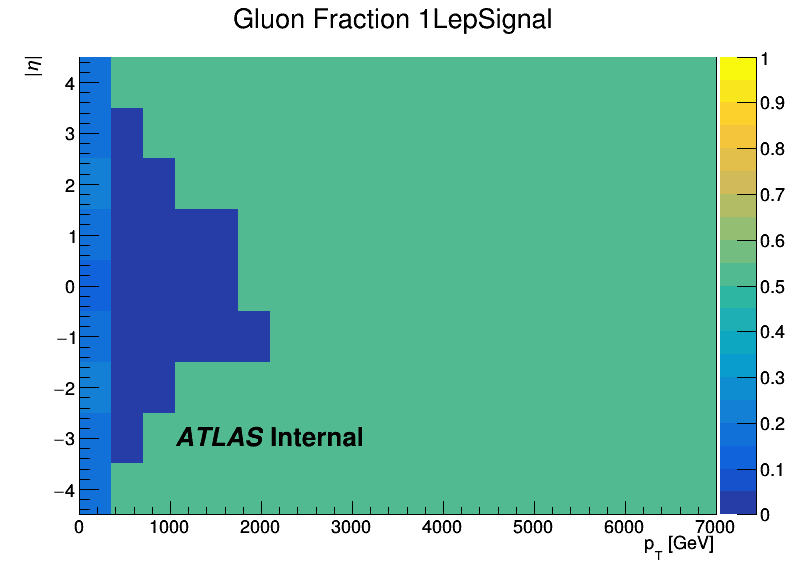
\includegraphics[width=\textwidth]{figures/QGfrac/GluonFrac2D_1LepSignal.png}
        \caption{Signal samples}
        \label{fig:GluonFracSignal}
    \end{subfigure}
    \hfill
    \begin{subfigure}[b]{0.3\textwidth}
        \centering
        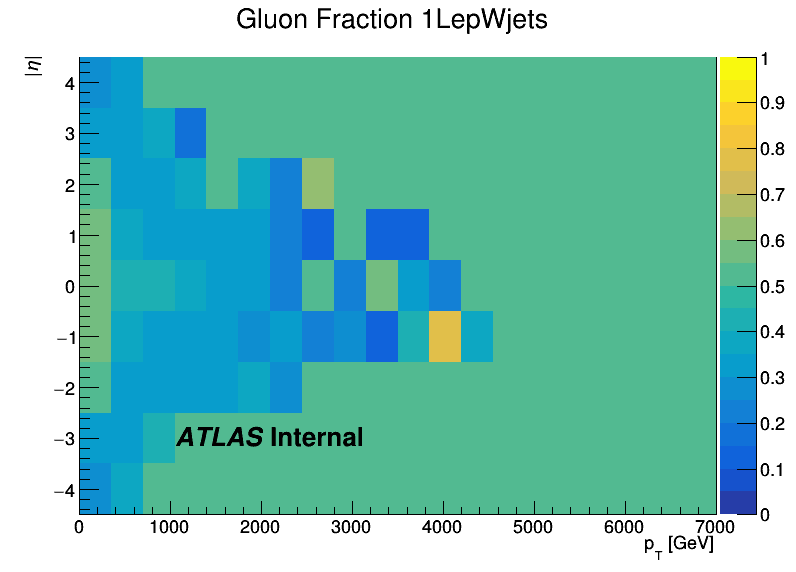
\includegraphics[width=\textwidth]{figures/QGfrac/GluonFrac2D_1LepWjets.png}
        \caption{\Wjets samples}
        \label{fig:GluonFracWjets}
    \end{subfigure}
    \hfill
    \begin{subfigure}[b]{0.3\textwidth}
        \centering
        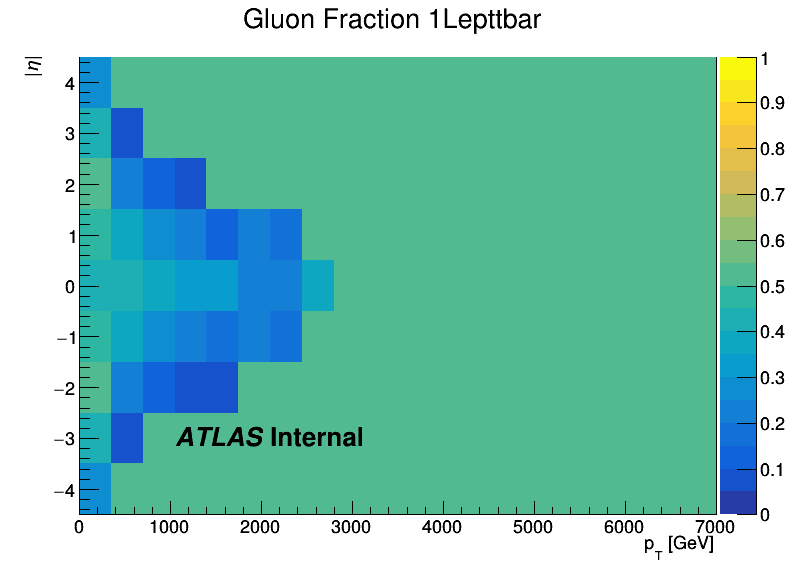
\includegraphics[width=\textwidth]{figures/QGfrac/GluonFrac2D_1Lepttbar.png}
        \caption{ttbar samples}
        \label{fig:GluonFracttbar}
    \end{subfigure}

    \bigskip

    \begin{subfigure}[b]{0.3\textwidth}
        \centering
        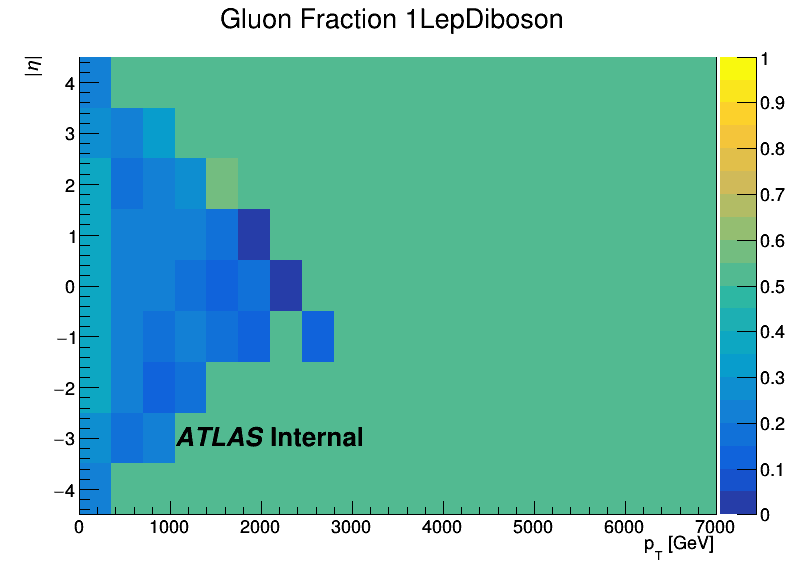
\includegraphics[width=\textwidth]{figures/QGfrac/GluonFrac2D_1LepDiboson.png}
        \caption{Diboson samples}
        \label{fig:GluonFracDiboson}
    \end{subfigure}
%    \hfill
    \begin{subfigure}[b]{0.3\textwidth}
        \centering
        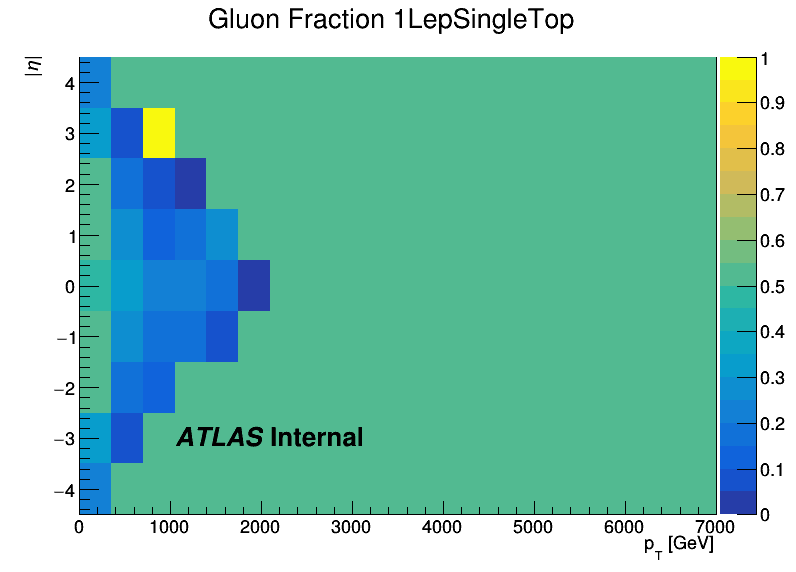
\includegraphics[width=\textwidth]{figures/QGfrac/GluonFrac2D_1LepSingleTop.png}
        \caption{Single top samples}
        \label{fig:GluonFracSingleTop}
    \end{subfigure}
    \hfill

    \caption{Gluon fraction inputs used to calculate jet uncertainties for the 1 lepton channel.}
    \label{fig:QGFracInputs2D1Lep}
\end{figure}


\begin{figure}[p]
    \centering
    \begin{subfigure}[b]{0.3\textwidth}
        \centering
        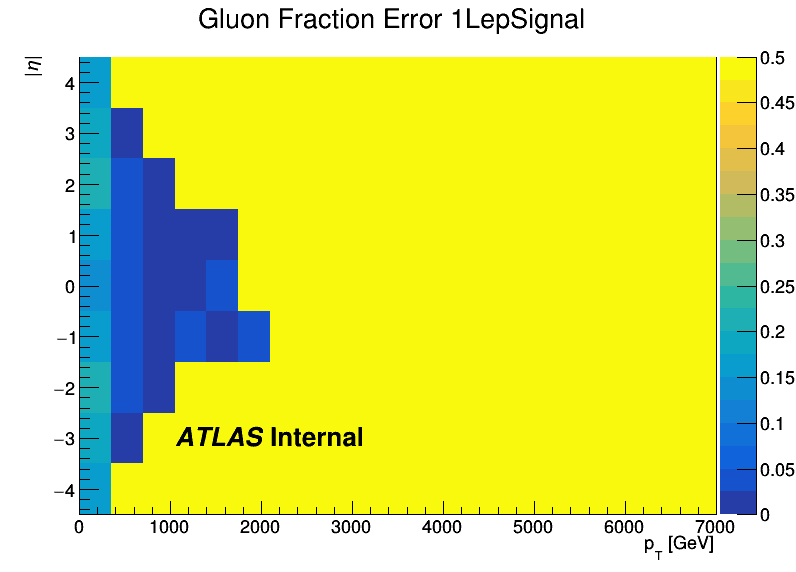
\includegraphics[width=\textwidth]{figures/QGfrac/GluonFracError2D_1LepSignal.png}
        \caption{Signal samples}
        \label{fig:GluonFracErrorSignal}
    \end{subfigure}
    \hfill
    \begin{subfigure}[b]{0.3\textwidth}
        \centering
        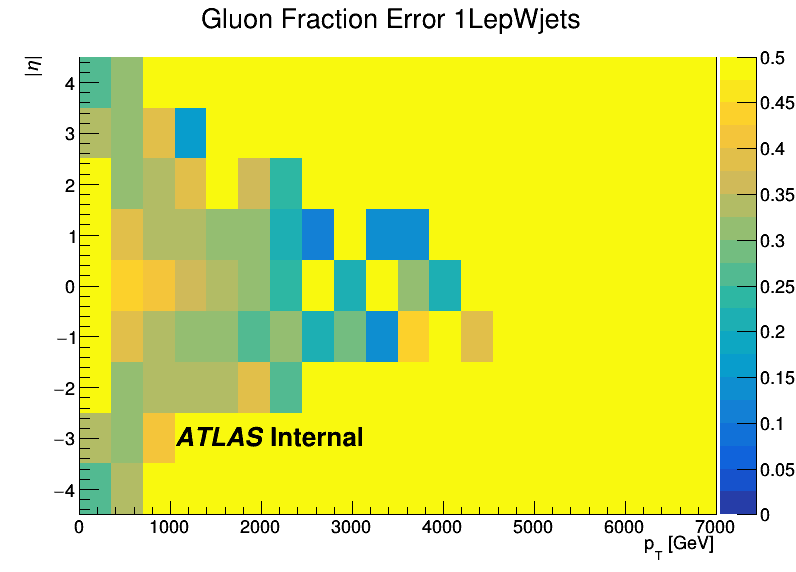
\includegraphics[width=\textwidth]{figures/QGfrac/GluonFracError2D_1LepWjets.png}
        \caption{\Wjets samples}
        \label{fig:GluonFracErrorWjets}
    \end{subfigure}
    \hfill
    \begin{subfigure}[b]{0.3\textwidth}
        \centering
        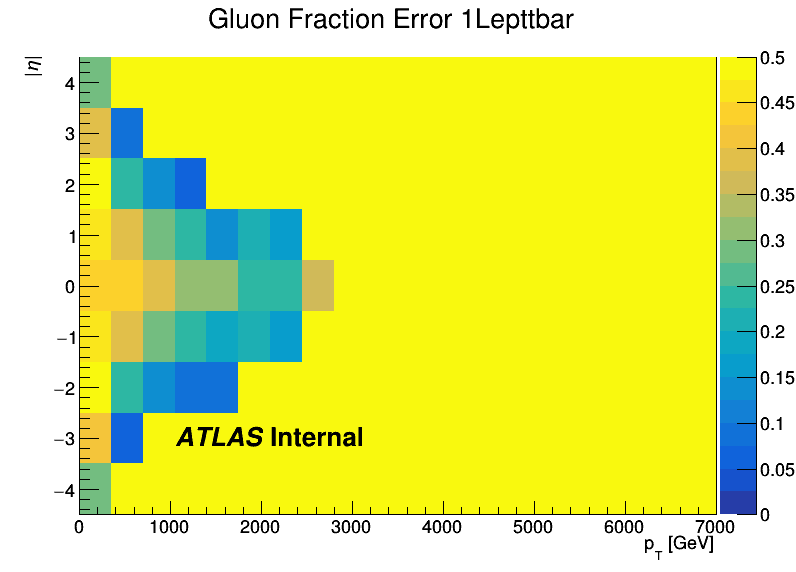
\includegraphics[width=\textwidth]{figures/QGfrac/GluonFracError2D_1Lepttbar.png}
        \caption{ttbar samples}
        \label{fig:GluonFracErrorttbar}
    \end{subfigure}

    \bigskip

    \begin{subfigure}[b]{0.3\textwidth}
        \centering
        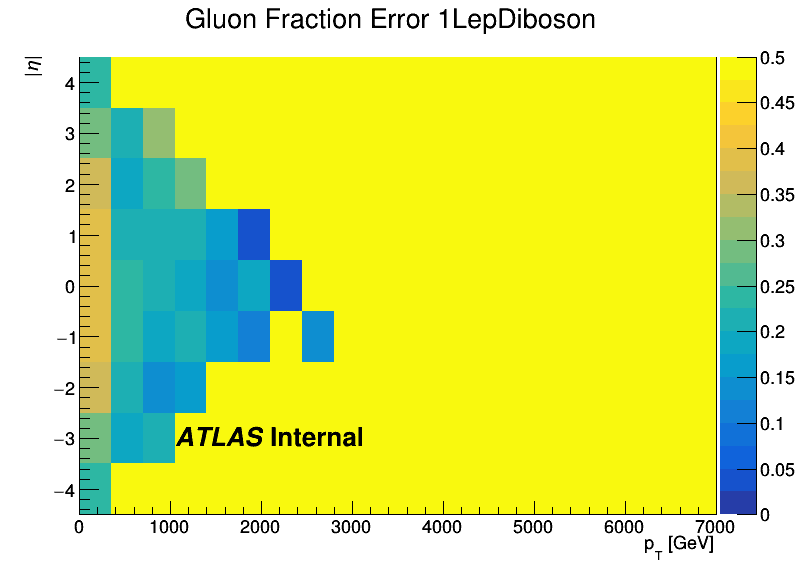
\includegraphics[width=\textwidth]{figures/QGfrac/GluonFracError2D_1LepDiboson.png}
        \caption{Diboson samples}
        \label{fig:GluonFracErrorDiboson}
    \end{subfigure}
%    \hfill
    \begin{subfigure}[b]{0.3\textwidth}
        \centering
        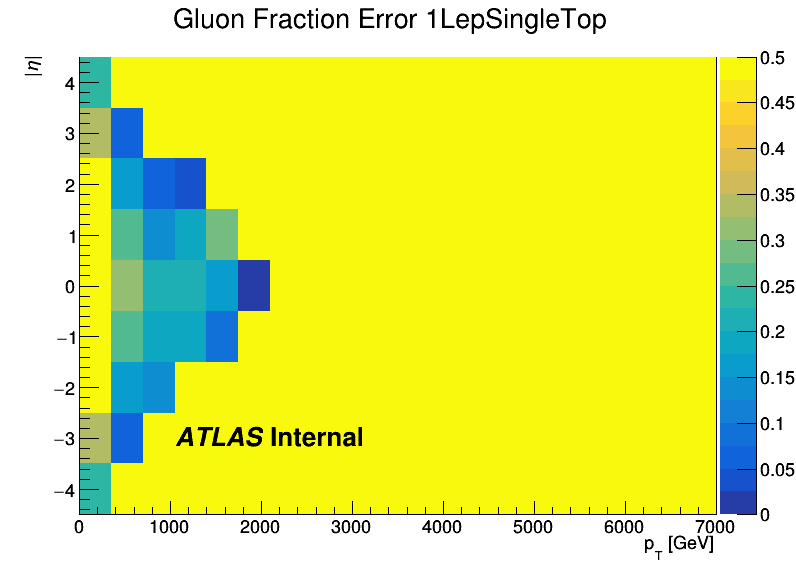
\includegraphics[width=\textwidth]{figures/QGfrac/GluonFracError2D_1LepSingleTop.png}
        \caption{Single top samples}
        \label{fig:GluonFracErrorSingleTop}
    \end{subfigure}
    \hfill

    \caption{Gluon fraction error inputs used to calculate jet uncertainties for the 1 lepton channel.}
    \label{fig:QGFracErrorInputs2D1Lep}
\end{figure}


\begin{figure}[ht]
    \centering
    \begin{subfigure}[b]{0.4\textwidth}
        \centering
        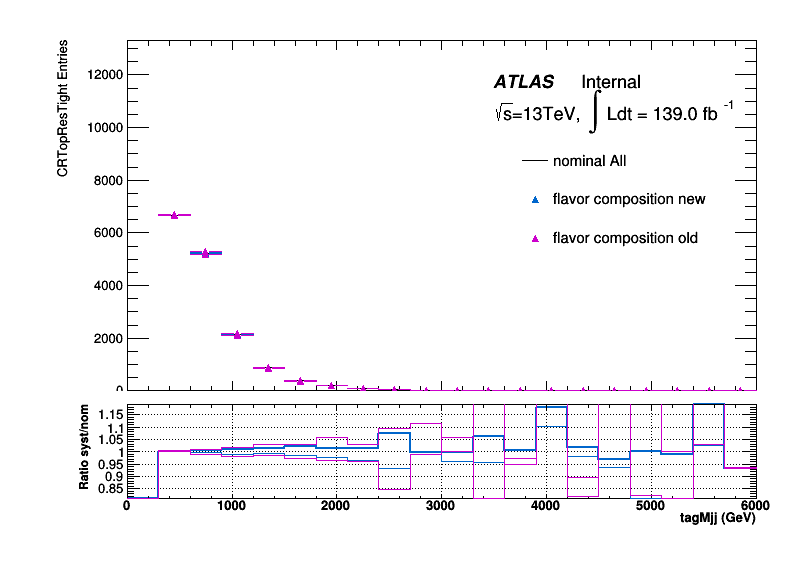
\includegraphics[width=\textwidth]{figures/1lep/FlavorVar/SystFCompCRTopResTight_All_tagMjj.png}
        \caption{Resolved TopCR Flavour Composition}
        \label{fig:ResolvedTopCRFlavourComposition}
    \end{subfigure}
    \quad % This adds some spacing between the figures in the same row
    \begin{subfigure}[b]{0.4\textwidth}
        \centering
        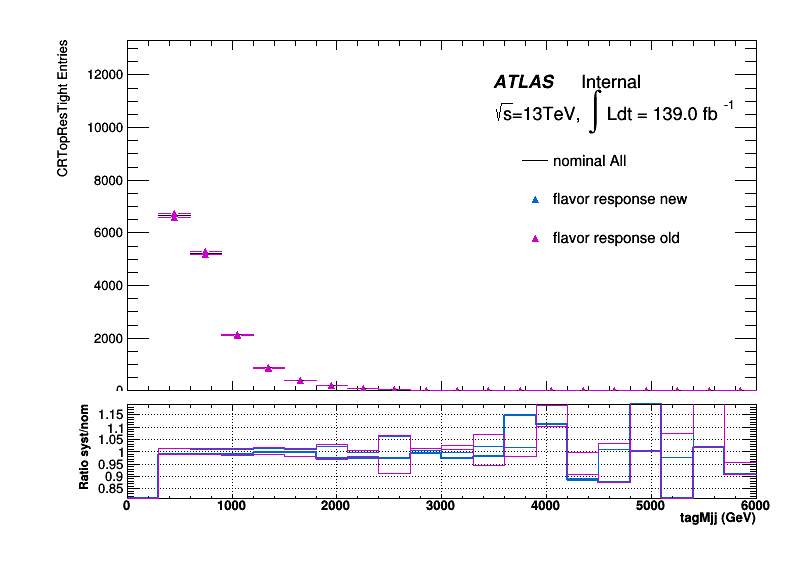
\includegraphics[width=\textwidth]{figures/1lep/FlavorVar/SystFResCRTopResTight_All_tagMjj.png}
        \caption{Resolved TopCR Flavour Response}
        \label{fig:ResolvedTopCRFlavourResponse}
    \end{subfigure}

    \bigskip % This adds extra vertical spacing between the rows of figures

    \begin{subfigure}[b]{0.4\textwidth}
        \centering
        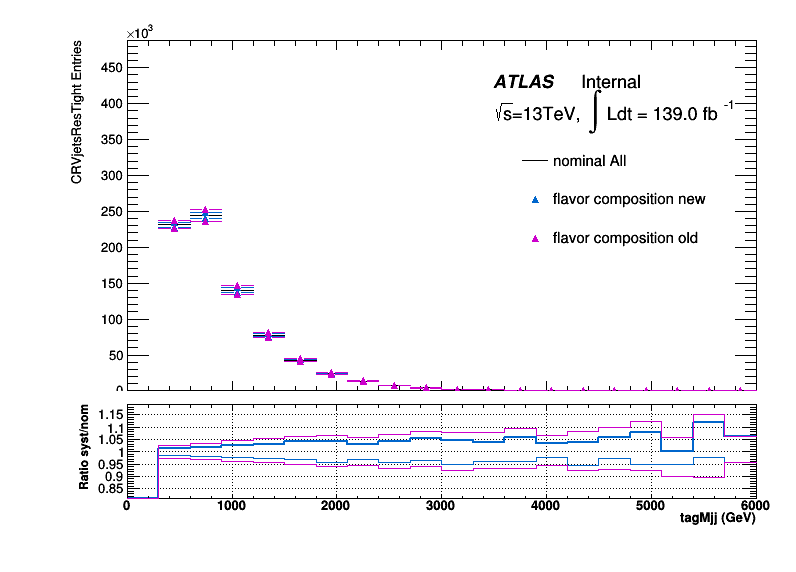
\includegraphics[width=\textwidth]{figures/1lep/FlavorVar/SystFCompCRVjetsResTight_All_tagMjj.png}
        \caption{Resolved WjetsCR Flavour Composition}
        \label{fig:ResolvedWjetsCRFlavourComposition}
    \end{subfigure}
    \quad % This adds some spacing between the figures in the same row
    \begin{subfigure}[b]{0.4\textwidth}
        \centering
        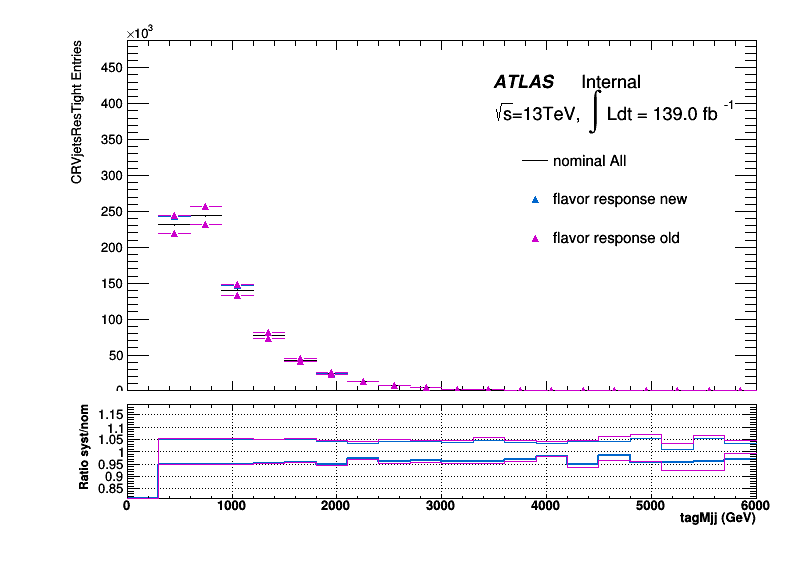
\includegraphics[width=\textwidth]{figures/1lep/FlavorVar/SystFResCRVjetsResTight_All_tagMjj.png}
        \caption{Resolved WjetsCR Flavour Response}
        \label{fig:ResolvedWjetsCRFlavourResponse}
    \end{subfigure}

    \caption{Comparison between old flavor uncertainties and newly derived flavor uncertainties.}
    \label{fig:1LepFlavorVarOldNew}
\end{figure}


% Flavour Variations for mc16a 1lep
%%%\begin{figure}[ht]
%%%    \centering
%%%        \subfigure[Resolved TopCR Flavour Composition]{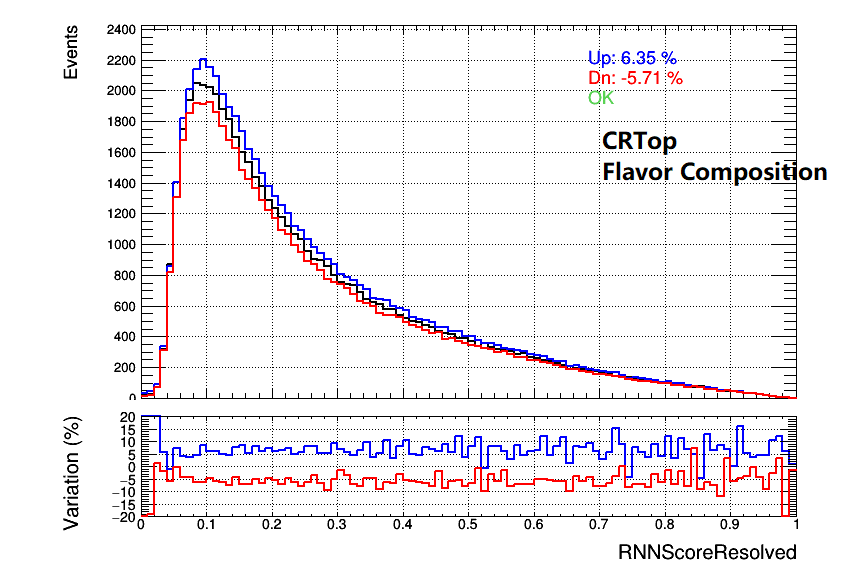
\includegraphics[width=0.4\textwidth]{figures/1lep/FlavorVar/C_0ptag2pjet_0ptv_CRTop_RNNScoreResolved_SysJET_Flavor_Composition.png}}
%%%        \subfigure[Resolved TopCR Flavour Response]{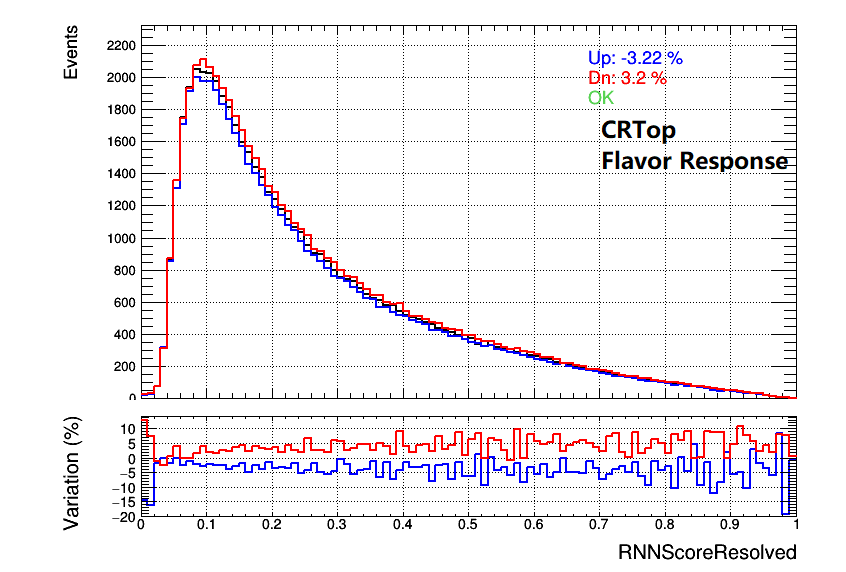
\includegraphics[width=0.4\textwidth]{figures/1lep/FlavorVar/C_0ptag2pjet_0ptv_CRTop_RNNScoreResolved_SysJET_Flavor_Response.png}}\\
%%%
%%%        \subfigure[Resolved WjetCR Flavour Composition]{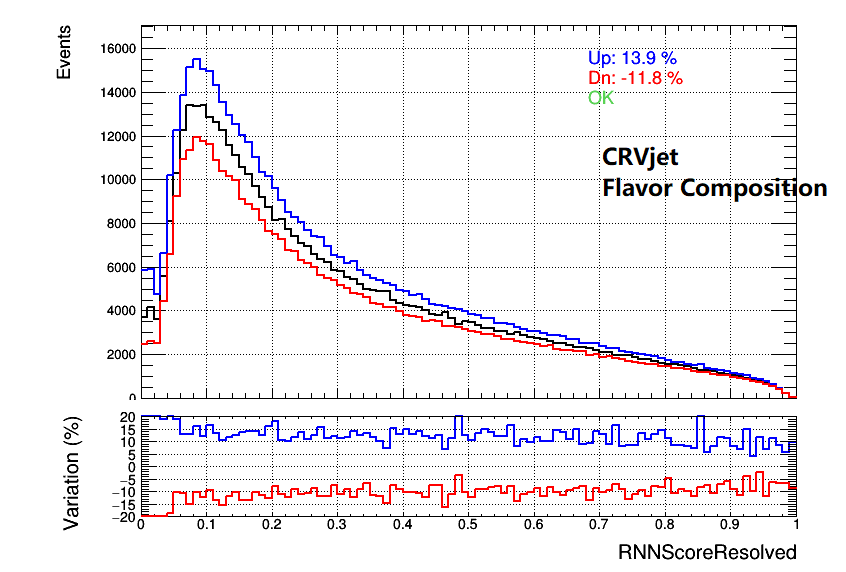
\includegraphics[width=0.4\textwidth]{figures/1lep/FlavorVar/C_0ptag2pjet_0ptv_CRVjet_RNNScoreResolved_SysJET_Flavor_Composition.png}}
%%%	\subfigure[Resolved WjetCR Flavour Reponse]{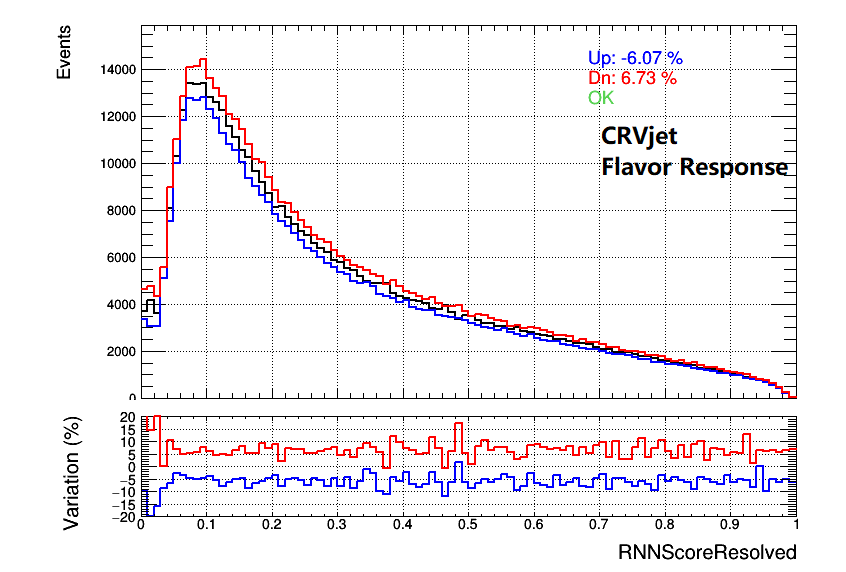
\includegraphics[width=0.4\textwidth]{figures/1lep/FlavorVar/C_0ptag2pjet_0ptv_CRVjet_RNNScoreResolved_SysJET_Flavor_Response.png}}
%%%
%%%        \caption{Impact of Flavour related variations on 1lepton resolved control regions. MC16A events are shown.}
%%%    \label{fig:1LepFlavorVariation}
%%%\end{figure}
%\begin{figure}[ht]
%    \centering
%        \subfigure[Resolved TopCR Flavour Composition]{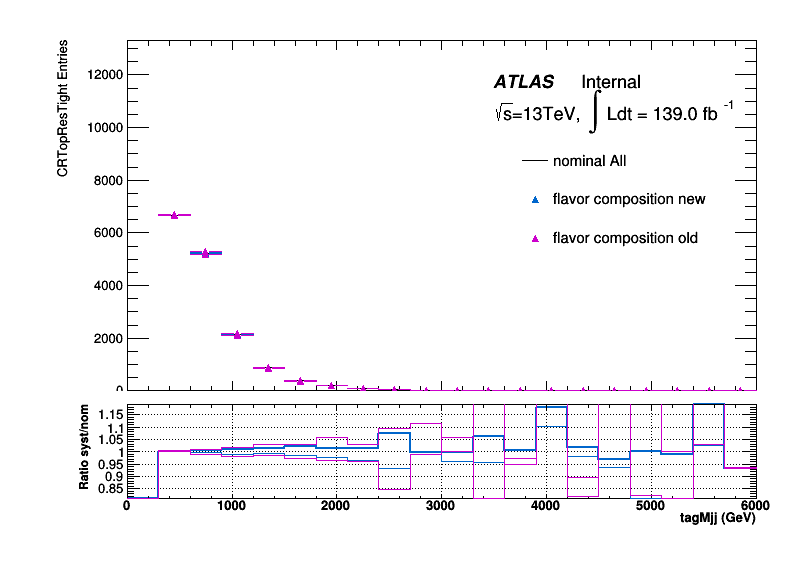
\includegraphics[width=0.4\textwidth]{figures/1lep/FlavorVar/SystFCompCRTopResTight_All_tagMjj.png}}
%        \subfigure[Resolved TopCR Flavour Response]{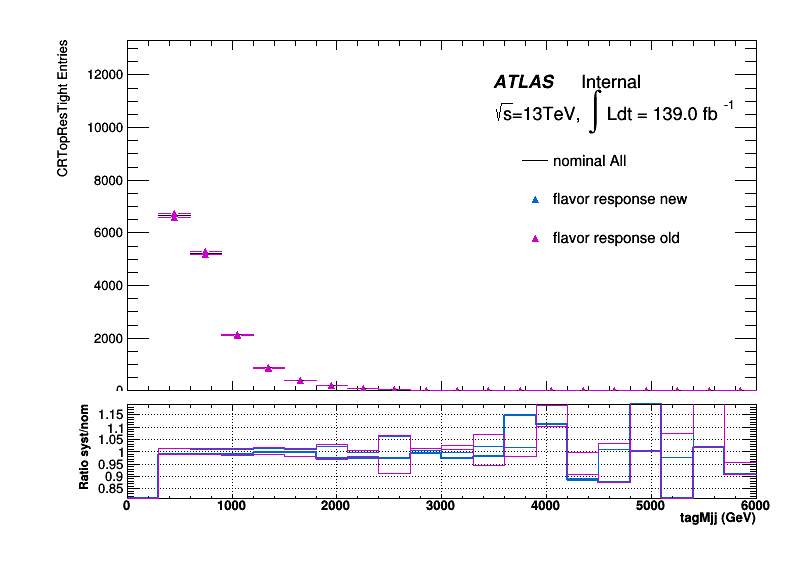
\includegraphics[width=0.4\textwidth]{figures/1lep/FlavorVar/SystFResCRTopResTight_All_tagMjj.png}} \\
%        \subfigure[Resolved WjetsCR Flavour Composition]{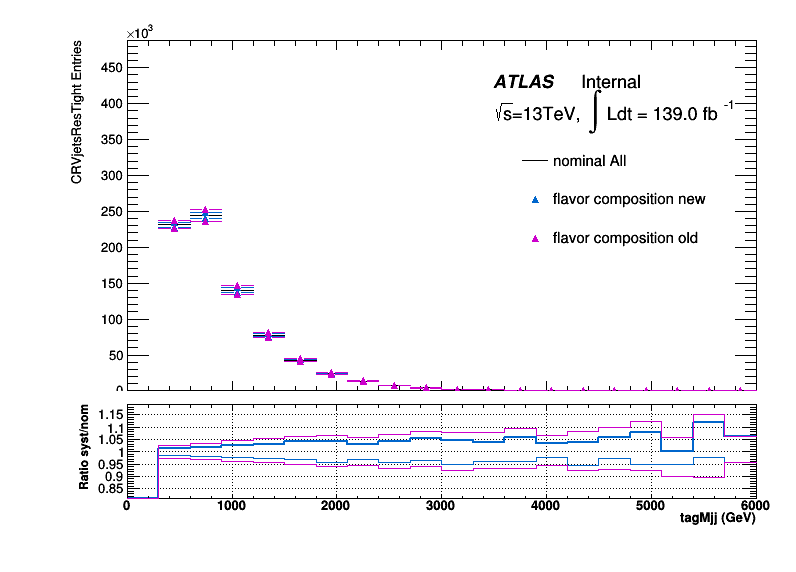
\includegraphics[width=0.4\textwidth]{figures/1lep/FlavorVar/SystFCompCRVjetsResTight_All_tagMjj.png}}
%        \subfigure[Resolved WjetsCR Flavour Reponse]{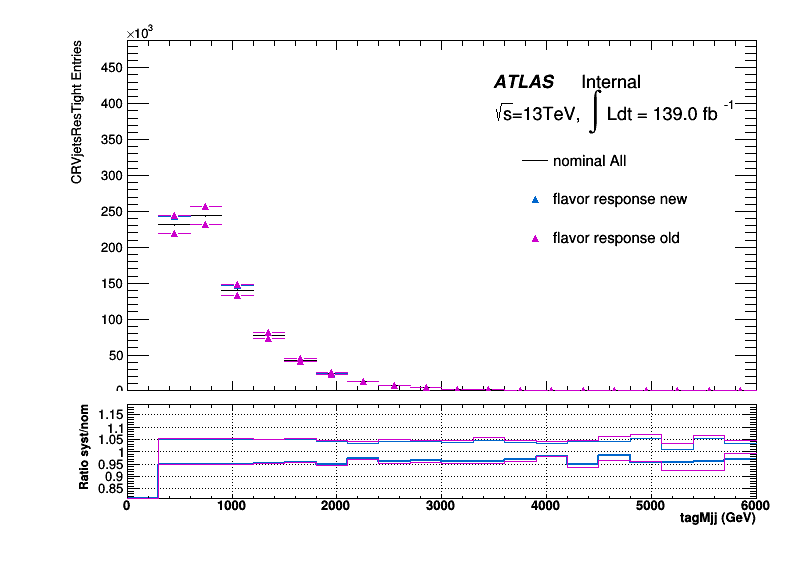
\includegraphics[width=0.4\textwidth]{figures/1lep/FlavorVar/SystFResCRVjetsResTight_All_tagMjj.png}}
%
%        \caption{Comparision between old flavor uncertainties and newly derived flavor uncertainties. Flavor composition uncertainties in particular are greatly reduced.}
%    \label{fig:1LepFlavorVarOldNew}
%\end{figure}



% Gluon fractions as function of pt for 2-lepton channel (nominal)

